\begin{frame}
    \frametitle{The analytic signal}
    \small
    
    \begin{figure}
        \centering
        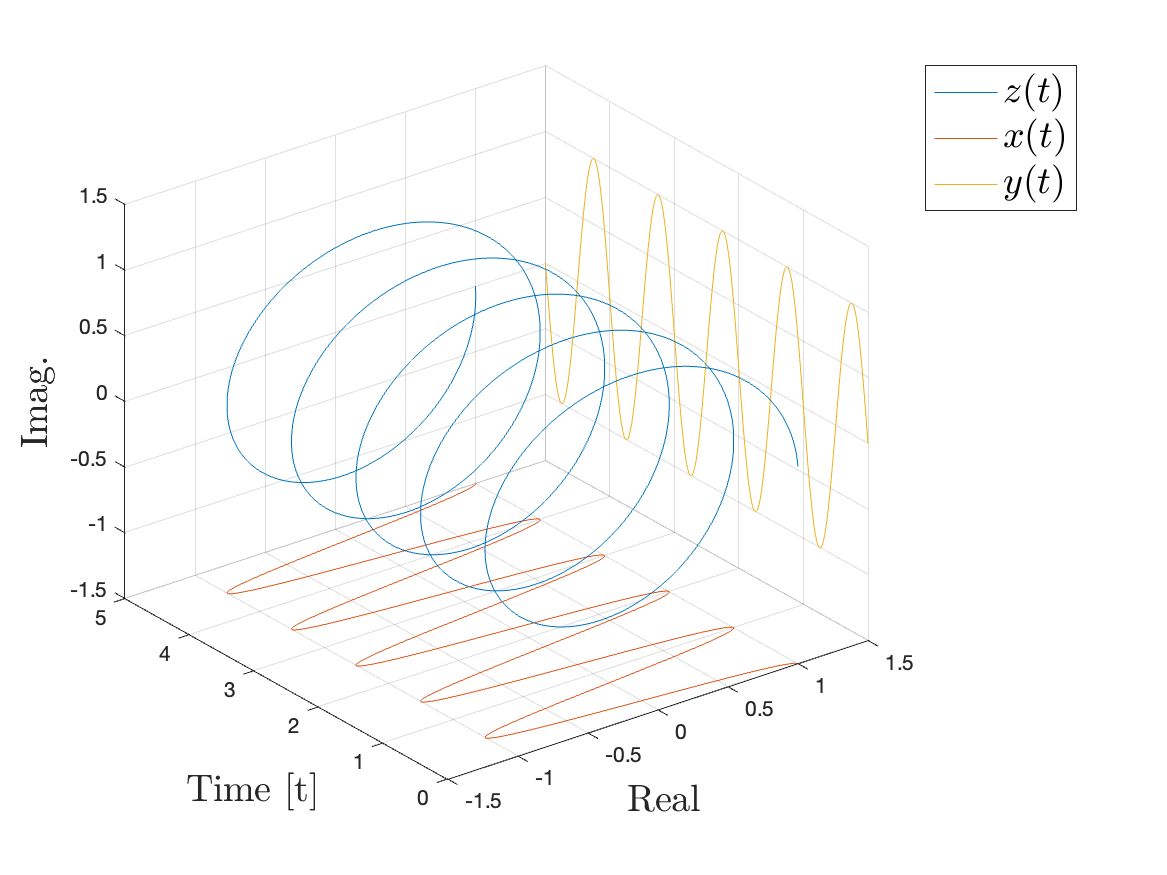
\includegraphics[width=0.75\textwidth]{images/analytic-signal.png}
        \caption{Analytic signal $z(t)$ of a real signal $x(t)=\cos(2\pi t)$, so that $z(t)=\cos(2\pi t) + j\sin(2\pi t)$ = 1 e^{j2\pi t}}
        \label{fig:spectrum}
    \end{figure}
   
\end{frame}
